\section{Degree}

\begin{frame}{Degree Theorem}
    \begin{theorem}[Degree Theorem \cite{Frieze_Karoński_2015}]
        Let $G$ be a random sparse graph. That is, $p = o(1)$. Now, let $\Delta(\mathcal{G}(n, p))$ and $\delta(\mathcal{G}(n, p))$ denotes the maximum and minimum degree of $\mathcal{G}(n, p)$, respectively, then
        \begin{enumerate}
            \item if $np = \omega \log n$ where $\omega \to \infty$, then w.h.p. 
            \[\delta(\mathcal{G}(n, p)) \approx \Delta(\mathcal{G}(n, p)) \approx np\]
            \item Let $p = c/n$ for some constant $c > 0$, then w.h.p
            \[\Delta(\mathcal{G}(n, p)) \approx \frac{\log{n}}{\log\log{n}}\]
        \end{enumerate}
    \end{theorem}
\end{frame}

\begin{frame}{Degree Theorem Proof - Warm Up}
    \setlength{\abovedisplayskip}{5pt}
    \setlength{\belowdisplayskip}{5pt}
    \setlength{\abovedisplayshortskip}{5pt}
    \setlength{\belowdisplayshortskip}{5pt}
    \begin{proof}[Degree Theorem - (i)]
        \begin{align*}
            \intertext{Let $X_i$ be an indicator random variable counting if edge $i^th$ connected to $u$ is presented or not, so.}
            X_i &= \begin{cases}
                1, \text{if $i$ is presented}\\
                0, \text{otherwise}
            \end{cases}
            \intertext{and,}
            X &= \sum_{i = 1}^{n - 1} X_i\\
            \intertext{Clearly, $X$ is binomial, so $\mathbb{E}[X] = (n - 1)p = O(np) \approx np$.}
        \end{align*}
    \end{proof}
\end{frame}

\begin{frame}{Degree Theorem Proof - Warm Up}
    \begin{figure}
        \centering
        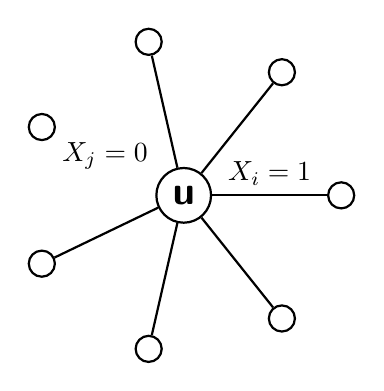
\begin{tikzpicture}[auto,node distance=2cm,
                    thick,main node/.style={circle,draw,font=\sffamily\Large\bfseries}]

          \node[main node] (1) {u};
        
          \foreach \place/\name in {{(0:2cm)/2}, {(51.428:2cm)/3}, {(102.856:2cm)/4}, {(154.284:2cm)/5}, {(205.712:2cm)/6}, {(257.14:2cm)/7}, {(308.568:2cm)/8}}
            \node[main node] (\name) at \place {};
        
          % Visible Edges
          \foreach \source/\target/\label in {1/2/$X_i = 1$, 1/3/ , 1/4/ , 1/6/ , 1/7/, 1/8/ }
            \path (\source) edge node[fill=white] {\label} (\target);
            
          \node at (-1,0.5) {$X_j = 0$};
        \end{tikzpicture}
        \caption{Degree Visualisation}
        \label{fig:degree-fig}
    \end{figure}
\end{frame}

\begin{frame}{Degree Theorem Proof - Warm Up}
    \setlength{\abovedisplayskip}{2pt}
    \setlength{\belowdisplayskip}{0pt}
    \setlength{\abovedisplayshortskip}{2pt}
    \setlength{\belowdisplayshortskip}{0pt}
    \begin{proof}[Degree Theorem - (i)]
        \begin{align*}
            \intertext{If $np = \omega\log{n}$ then}
            \textbf{Pr}[\exists v: |\deg(v) - np| \geq \delta np] &\leq 2\exp\left\{-\frac{\omega^{-2/3}np}{3}\right\} = 2\exp\left\{-\frac{\omega^{1/3}\log{n}}
            {3}\right\} = \frac{2}{n^{\omega^{1/3}/3}}\\
            \intertext{Thus,}
            \textbf{Pr}[\forall v: |\deg(v) - np| < \delta np] &\geq 1 - O\left(n^{-\omega^{1/3}/3}\right)
            \intertext{which occurs with high probability. Hence,}
        \end{align*}
        \[\delta(\mathcal{G}(n, p)) \approx \Delta(\mathcal{G}(n, p)) \approx np\]
    \end{proof}
\end{frame}

\begin{frame}{Degree Theorem Proof}
    \setlength{\abovedisplayskip}{2pt}
    \setlength{\belowdisplayskip}{0pt}
    \setlength{\abovedisplayshortskip}{2pt}
    \setlength{\belowdisplayshortskip}{0pt}
    \begin{proofs}[Degree Theorem - (ii) Case 1 / Case 2]
        \begin{align*}
            \intertext{We will prove the upper and lower bounds on $d$. Let $d^- = \ceil{\frac{\log{n}}{\log\log{n} - 2\log\log\log{n}}}$, then,}
            \textbf{Pr}[\exists v: \deg(v) \geq d] &\leq n {{n - 1} \choose d} \left(\frac{c}{n}\right)^d\\
            \intertext{recall from many classes that ${{n - 1} \choose d} \leq \left(\frac{en}{d}\right)^d$, so}
            &\leq n\left(\frac{ec}{d}\right)^d = \frac{e^{\log n} \cdot e^d \cdot e^{d\log{c}} }{e^{d\log{d}}}\\
            &= \exp\left\lbrace \log{n} - d\log{d} + d + d\log{c}\right\rbrace = \exp\left\lbrace \log{n} - d\log{d} + O(d)\right\rbrace\\
            &\leq \exp\left\lbrace \log{n} - \log{n}\log{\log{n}} + O(\ceil{\frac{\log{n}}{\log\log{n} - 2\log\log\log{n}}})\right\rbrace\\
            &\leq \exp\left\lbrace-\log{n}\log{\log{n}} + O(\log{n})\right\rbrace = \exp\left\lbrace \log{n}\left(O(1) -\log{\log{n}}\right)\right\rbrace\\
            &\leq \exp\{-\log{n}\} = 1/n
        \end{align*}
    \end{proofs}
\end{frame}

\begin{frame}{Degree Theorem Proof}
    \setlength{\abovedisplayskip}{2pt}
    \setlength{\belowdisplayskip}{0pt}
    \setlength{\abovedisplayshortskip}{2pt}
    \setlength{\belowdisplayshortskip}{0pt}
    \begin{proofs}[Degree Theorem - (ii) Case 1 / Case 2]
        \[\textbf{Pr}[\forall v: \deg(v) < d^-] \geq 1 - \frac{1}{n}\]
        \begin{align*}
            \intertext{with high probability. Now on to case 2, let $d^+ = \ceil{\frac{\log{n}}{\log\log{n} + 2\log\log\log{n}}}$ and $X_d$ be the number of vertices of degree $d$, and $X_{d, i}$ be respective Bernoulli r.v in $\mathcal{G}(n, p)$, then}
            \mathbb{E}[X_d] &= \sum_{i \in I} \textbf{Pr}[X_{d, i} = 1] = \sum_{i \in I} \left(\frac{c}{n}\right)^d \left(1 - \frac{c}{n}\right)^{n - d - 1} = n{{n - 1} \choose d}\left(\frac{c}{n}\right)^d \left(1 - \frac{c}{n}\right)^{n - d - 1}\\
            &= \exp\left\{\log{n} - \frac{\log{n}}{\log{\log{n}}}(\log\log{n} - \log\log\log{n} + o(1)) + O(d)\right\} \to \infty
            \intertext{From here, the text also went to infinity and beyond and skipped directly to the results. So whatever comes after is from a fragment of my imagination adapting from another special case from another Theorem.}
        \end{align*}
    \end{proofs}
\end{frame}

\begin{frame}{Degree Theorem Proof}
    \begin{proofs}[Degree Theorem - (ii) Case 2]
        \setlength{\abovedisplayskip}{2pt}
        \setlength{\belowdisplayskip}{0pt}
        \setlength{\abovedisplayshortskip}{2pt}
        \setlength{\belowdisplayshortskip}{0pt}
        \begin{align*}
            \intertext{Let's first do some acrobatics. Notice that,}
            {{n - 1} \choose d} &= \frac{(n - 1)!}{d!(n - d)!} = \frac{(n - 1)(n - 2)(n - 3)...(n - d) }{d!} = \frac{\prod_{i = 1}^{d - 1}(n - i) }{d!}\\
            \intertext{Consider the first few expansions of the numerator, we get}
            \prod_{i = 1}^{d}(n - i) &= n^{d} - \left(\sum_{ i = 1}^{d} i\right) \cdot n^{d - 1} + (\cdot)O\left(n^{d - 2}\right) + \hdots\\ 
            &= n^{d} + O(d^2)n^{d - 1} + O(n^{d - 2}) + \hdots\\
            &= n^{d}\left[1 - O(d^2)O(1/n) + O(d^3)O(1/n^2) + \hdots\right]\\
            &= n^{d}\left[1 + O(d^2)O(1/n)\right] = n^d\left[1 + O\left(\frac{d^2}{n}\right)\right]
        \end{align*}
    \end{proofs}
\end{frame}

\begin{frame}{Degree Theorem Proof}
    \begin{proofs}[Degree Theorem - (ii) Case 2]
        \setlength{\abovedisplayskip}{2pt}
        \setlength{\belowdisplayskip}{0pt}
        \setlength{\abovedisplayshortskip}{2pt}
        \setlength{\belowdisplayshortskip}{0pt}
        \begin{align*}
            \mathbb{E}[X_d] &= n{{n - 1} \choose d}\left(\frac{c}{n}\right)^d \left(1 - \frac{c}{n}\right)^{n - d - 1}\\
            &= n \frac{n^d}{d!}\left(1 + O\left(\frac{d^2}{n}\right)\right)\left(\frac{c}{n}\right)^d \exp\left\{-(n - 1 - d)\left(\frac{c}{n} + O\left(\frac{1}{n^2}\right)\right)\right\}\\
            &= n\frac{c^d}{d!}\left(1 + O\left(\frac{d^2}{n}\right)\right)\exp\left\{-c + O\left(\frac{1}{n}\right) + \frac{c}{n} + \frac{1}{n^2}-\frac{cd}{n} + O\left(\frac{d}{n^2}\right)\right\}\\
            &= n\frac{c^d}{d!}\left(1 + O\left(\frac{d^2}{n}\right)\right)\exp\left\{O\left(\frac{1}{n}\right) + (1 - d)\frac{c}{n} + O\left(\frac{d}{n^2}\right)\right\}\\
            &= n\frac{c^de^{-d}}{d!}\left(1 + O\left(\frac{1}{n}\right)\right)\\
            &= O(n)\\
        \end{align*}
    \end{proofs}
\end{frame}


\begin{frame}{Degree Theorem Proof}
    \setlength{\abovedisplayskip}{2pt}
        \setlength{\belowdisplayskip}{0pt}
        \setlength{\abovedisplayshortskip}{2pt}
        \setlength{\belowdisplayshortskip}{0pt}
    \begin{proofs}[Degree Theorem - (ii) Case 2]
        \begin{align*}
            \intertext{We now compute the following quantity,}
            \textbf{Pr}[\deg(u) = \deg(v) = d] &= \frac{c}{n}\left({{n - 2} \choose {d - 1}}\left(\frac{c}{n}\right)^{d - 1}\left(1 - \frac{c}{n}\right)^{n - 1 - d}\right)^2\\
            &+ \left(1 - \frac{c}{n}\right)\left({{n - 2} \choose d}\left(\frac{c}{n}\right)^d\left(1 - \frac{c}{n}\right)^{n - 2-d}\right)^2
            \intertext{First line takes care of where there is an edge between $u$ and $v$, and the second is there when there isn't. So}
            &= \textbf{Pr}[\deg(u) = d]\textbf{Pr}[\deg(v) = d]\left(1 + O\left(\frac{1}{n}\right)\right)
        \end{align*}
    \end{proofs}
\end{frame}

\begin{frame}{Degree Theorem Proof}
    \setlength{\abovedisplayskip}{2pt}
        \setlength{\belowdisplayskip}{0pt}
        \setlength{\abovedisplayshortskip}{2pt}
        \setlength{\belowdisplayshortskip}{0pt}
    \begin{proofs}[Degree Theorem - (ii) Case 2]
        \begin{align*}
            \intertext{Recall that $Var(X) = \mathbb{E}[(X - \mu)^2] = \mathbb{E}[X^2] - \mathbb{E}[X]^2$, so}
            \mathbb{E}\left[\left(\sum_{i = 1}^n X_i\right)^2\right] &= \mathbb{E}\left[\sum_{i = 1}^n \sum_{j = 1}^n X_iX_j\right]  = \sum_{i = 1}^n \sum_{j = 1}^n\mathbb{E}\left[X_iX_j\right] = \sum_{i = 1}^n \sum_{j = 1}^n\textbf{Pr}[X_i = d, X_j = d]\\
            \intertext{Now,}
            \mathbb{E}[X]^2 &= \left(\sum_{i = 1}^n\textbf{Pr}[X_i = d]\right)\left(\sum_{j = 1}^n\textbf{Pr}[X_j = d]\right) = \sum_{ i =1}^n \sum_{j = 1}^n \textbf{Pr}[X_i = 1] \textbf{Pr}[X_j = d]\\
            \intertext{So,}
            \text{Var}(X_d) &= \sum_{ i =1}^n \sum_{j = 1}^n \left[\textbf{Pr}[X_i = d, X_j = d] - \textbf{Pr}[X_i = 1] \textbf{Pr}[X_j = d]\right] = \sum_{i = 1}^n\sum_{j = 1}^n \text{Cov}(X_i, X_j)
        \end{align*}
    \end{proofs}
\end{frame}

\begin{frame}{Degree Theorem Proof}
    \setlength{\abovedisplayskip}{2pt}
        \setlength{\belowdisplayskip}{0pt}
        \setlength{\abovedisplayshortskip}{2pt}
        \setlength{\belowdisplayshortskip}{0pt}
    \begin{proofs}[Degree Theorem - (ii) Case 2]
        \begin{align*}
            \intertext{Substituting in earlier results yields,}
            \text{Var}(X_d) &= \sum_{ i =1}^n \sum_{j = 1}^n \left[\textbf{Pr}[\deg(u) = d]\textbf{Pr}[\deg(v) = d]\Big(1 + O\left(\frac{1}{n}\right)\right) \\
            &\qquad \qquad \qquad \qquad \qquad- \textbf{Pr}[\deg(u) = d]\textbf{Pr}[\deg(v) = d]\Big]\\
            &= \sum_{i \neq j = 1}^n \left[\textbf{Pr}[\deg(u) = d]\textbf{Pr}[\deg(v) = d]O\left(\frac{1}{n}\right)\right] + \sum_{i = j}^n \text{Cov}(X_i, X_i)\\
            &= \sum_{i \neq j = 1}^n \left[\textbf{Pr}[\deg(u) = d]\textbf{Pr}[\deg(v) = d]O\left(\frac{1}{n}\right)\right] + \sum_{i = j}^n \text{Var}(X_i)
        \end{align*}
    \end{proofs}
\end{frame}

\begin{frame}{Degree Theorem Proof}
    \setlength{\abovedisplayskip}{2pt}
        \setlength{\belowdisplayskip}{0pt}
        \setlength{\abovedisplayshortskip}{2pt}
        \setlength{\belowdisplayshortskip}{0pt}
    \begin{proofs}[Degree Theorem - (ii) Case 2]
        \begin{align*}
            \intertext{Variance of indicator (Bernoulli) is just $pq$, so}
            \text{Var}(X_d)&\leq \sum_{i \neq j = 1}^n O\left(\frac{1}{n}\right) + \sum_{i = j}^n \textbf{Pr}[X_i = d](1 - \textbf{Pr}[X_i = d])\\
            \intertext{Since $0 < p, q, < 1$ and $\mathbb{\mathcal{\mathbbm{1}}} = p$, $\text{Var}(\mathcal{\mathbbm{1}}) < \mathbb{E}[\mathbbm{1}]$, hence}
            &\leq \sum_{i \neq j = 1}^n O\left(\frac{1}{n}\right) + \mathbb{E}[X]\\
            &= \sum_{i = 1}^n \sum_{j \neq i}^n O\left(\frac{1}{n}\right) + \mathbb{E}[X]\\
            &= O(n) + O(n)\\
            &= O(n)
        \end{align*}
    \end{proofs}
\end{frame}

\begin{frame}{Degree Theorem Proof}
    \setlength{\abovedisplayskip}{2pt}
        \setlength{\belowdisplayskip}{0pt}
        \setlength{\abovedisplayshortskip}{2pt}
        \setlength{\belowdisplayshortskip}{0pt}
    \begin{proof}[Degree Theorem - (ii) Case 2]
        \begin{gather*}
            \intertext{Using Chebyshev's,}
            \textbf{Pr}[X_d = 0] \leq \textbf{Pr}[|X_d - \mathbb{E}[X_d]| \geq \mathbb{E}[X_d]] \leq \frac{\text{Var}(X_d)}{(\mathbb{E}[X])^2} \leq \frac{O(n)}{(O(n))^2} \leq O\left(\frac{1}{n}\right)\
            \intertext{Hence,}
            \textbf{Pr}[X_d > 0] \geq 1 -  O\left(\frac{1}{n}\right)
            \intertext{Which occurs with high probability. From these two, we get that $\forall v \in G, \deg(v) < d^-$, and $\exists u \in G: \deg(u) > d^+$, so}
            \frac{\log{n}}{\log\log{n} + \log\log\log{n}}\leq \deg(u) \leq \frac{\log{n}}{\log\log{n} - 2\log\log\log{n}}\\
            \Omega\left(\frac{\log{n}}{\log\log{n}}\right) \leq \deg(u) \leq O\left(\frac{\log{n}}{\log\log{n}}\right)
        \end{gather*}
    \end{proof}
\end{frame}
